\chapter{Design and Methodology}

\section{The Simulator}
In order to understand propagation and the scalability of the dash network, a
simulator was developed at ASU using an already existing simulator that was
developed at ETH Zurich for this research \citep{eth}
 
 The ETH blockchain simulator is an NS3 (Network Simulator 3) based bitcoin simulator. This
 simulator demonstrates the workings of Bitcoin, Dogecoin and Litecoin, but
 bases its research on each block being the fundamental/rudimentary component. 

 We found that simulations that merely went down to the block level were not
 detailed enough for our purpose. In order to reliably model a consensus
 network with block propagation speedups such as compact or xthin we must
 understand these networks down at the level of transactions.

 In order to understand the network at the level of transactions, we modeled
 generation of transactions using a normal
 distribution. Each node is has a transaction generator that creates a random
 transaction with a piecewise constant
 distribution and hashes that data.

 Masternode in the current simulator is not a separate class but a check on
 full node.  The network is randomly distributed with full nodes, masternodes
 and the miners. All the miners in the network are connected to each other
 which simulates the real world network.  When establishing the connections
 between nodes, we create point-to-point channels between them, which abstracts
 away any intermediate devices (routes, switches, etc). These channels have two
 characteristics: 

\begin{enumerate}
    \item Latency
    \item Bandwidth
\end{enumerate}

Mining pools typically maintain private peering connections among
themselves which we capture in our simulations. 

In short, below are the modifications done to the bitcoin-simulator for it to
run the current dash-simulations:


\begin{enumerate}
    \item Transactions are added in order to add traffic and understand
        propagation techniques in more detail.
    \item Every node now has its own mempool in order to test set reconciliation
        for Xthin and Compact propagation.
    \item Compact block propagation is added.
    \item Extreme thin block propagation is added.
    \item Masternode (bool) is added to the full-node. Because this is network
        propagation, the bandwidth is the only differentiating factor between a
        full node and masternode.
    \item Bloom filter using Murmur Hash library is added in order to test
        xthin.
    \item Capability to test x-11 hashing is added, although it doesn't add
        value to propagation.
    \item FillBlock - this parameter if true, fills the block with transactions
        to its maximum capacity. If this is set to false, the simulator uses a
        piecewise constant distribution to generate the next block size and adds
        transactions limiting to the new block size.
\end{enumerate}

The resulting simulator code is available at \cite{nakul}

\subsection{Parameters}
The simulator takes in the below given parameters:

\begin{enumerate}
    \item Block size
    \item Block Interval
    \item Propagation type
    \item Number of blocks
    \item Fill block - The block is filled to capacity if fillBlock=true.
\end{enumerate}

We ran multiple experiments in order to understand and compare the below three
types of propagation:

\begin{enumerate}
    \item Traditional
    \item Compact
    \item Extreme Thin Blocks
\end{enumerate}

The simulations were run with different network sizes and different block sizes.
Through these simulations, it was realized that both compact and xthin blocks
can support the Dash network with a capacity an order of magnitude larger than
the traditional block propagation.

We ran simulations for both Compact and XThin in the same testing set up from
block sizes of 1 MB to 10MB. 
Through the experiments, we were able to observe that compact blocks are not
scalable above 4MB block sizes on the dash network. However, we were able to
propagate XThin blocks with lower orphan rates.
The reason XThin blocks gave us better results is because of the bloom filter
that is sent apart from cheap hashes, which helps understand the other peer
whether or not what full transactions to send.

\textbf{Note:} The simulator does not always present the same results every time because the propagation can take different routes, the distributions used can use different node bandwidths, blocks are generated using Geometric progression from a seed value which is generated from a random seed. Parameters and distributions used in the simulator, gives some variance to the results, although the increase/decrease slope of the results can be confidently used.


\section{Hypothesis}
The memory pools of the nodes on the network are not synchronized when there is
high amount of transaction flow. This is because of the following reasons:


\begin{enumerate}
    \item Unspent transactions that are relayed to the node are stored
        in-memory. When transactions flow is high, and the memory is full, the
        transactions are dropped.
    \item Transactions use gossip protocol for propagation through the decentralized network and therefore rely on nodes that are forwarding it. It is not always possible for the transaction to have relayed to a node where the block is received. Since, compact, XThin and graphene rely on memory pool synchronization, it is not always the case that all transactions relayed in the block sketch are known to the node. 
\end{enumerate}

Since, the memory pools of the peers go out of sync, reducing payload by using
cheap hashes often leads to re-transmissions. This re-transmission is in the
form of complete block or block transactions. In order to increase the speed of
this request, we use fountain codes. Using fountain codes enables reliable
transmission of data between all peer nodes and then aggregating the data at the
node that is requesting the block.

The reasons of using and applying them to blockchains for transmitting data are
multifold:

\begin{enumerate}
    \item The primary reason for using fountain (raptor) codes is
     that they work on quantity (\texttt{k}) of symbols rather than quality (what part of data is being relayed). Therefore, on receiving any \texttt{k} symbols, we can reconstruct a block with 99.5\% efficiency \citep{fountain-pres} .
     
    \item Infinite decoding symbols can be created using the data, all
        peers required to send the data create k/(number of peers) symbols, independent of what the
        other peers have created, and then send them to the receiving node to
        reconstruct the block.
    \item On decode failures, creating more decode or repair symbols has a
        linear complexity therefore these symbols are not compute heavy.
    \item The repair symbols are small in size and can be relayed faster rather
        than sending the whole block for recovery. 
\end{enumerate}

The most important among others for us is that they are computationally easier to
encode/decode since they use binary operations for both and they are server independent. In case
of blockchains, we can ask data from all connected peer nodes and
collect symbols to recreate the block. This will generate a lower upload
footprint for the nodes that are serving data therefore leads to a faster
synchronization. 
The scalability can be tested by using this propagation technique for large block sizes till 
we lose consensus (Orphan rate = 50\%). The block propagation throughput is constrained by orphan rate of the network.

\section{The protocol specifications}

Below are the specifications of the implementation of protocol used by digital
fountain in blockchains:

\begin{enumerate}
    \item The sender node, on hearing a new block, sends an inv to another peer.
        The whole block body is reinterpreted as a byte array and then encoded
        into a set of symbols of a length that was negotiated between the peers.

    \item On receiving the inv/header message the receiver requests the whole
        blocks using an expedited \texttt{getraptor} request to \textbf{all its
        peers}.
    \item All peers who have heard of the block respond with \texttt{raptorcode}
        and encoded symbols of the blocks. The other peers drop the message.
    \item The receiver collects these symbols in a singleton class (map of block 
        header ID to symbol ID and symbol pair). Note that, since this research
        is done for large block sizes, symbols here will be significantly large.
        In order to prevent DoS attacks, every symbol must contain the header.
        The header should not be encoded. In smaller blocks, this can be
        optimized to send only the 64 byte hash along with every symbol.
    \item The receiver knows the amount of symbols needed to reconstruct the
        block and waits till it gets at least the required count of the symbols.
    \item On reaching the required count, it reconstructs the block using raptor
        decoding and serializes the stream on byte array to form the block.
\end{enumerate}

The above is also shown in the figure \ref{image: protocol}

\begin{figure}
    \captionsetup{justification=centering}
    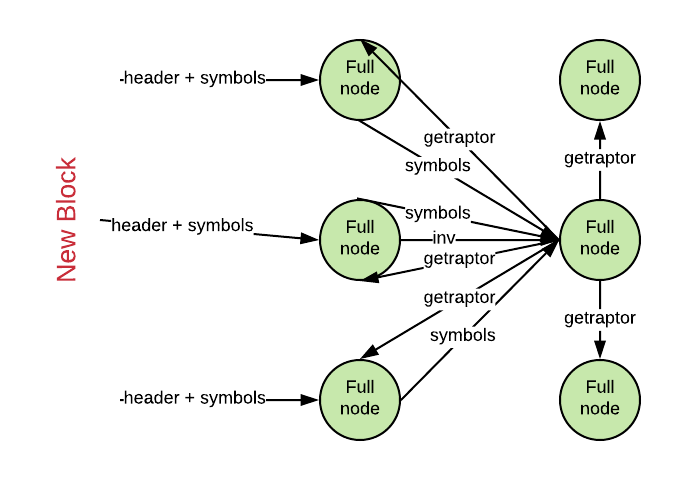
\includegraphics[width=1\columnwidth, height=.7\columnwidth]{files/protocol.png}
     \centering
     \caption{Protocol}
     \label{image: protocol}
\end{figure}

\section{Implementation Details}

The implementation in order to test the hypothesis of data aggregation is done
in 2 parts:

\begin{enumerate}
    \item \textbf{Dash Core Client:}In this specific implementation, the
        following parts are implemented:

        \begin{enumerate}
            \item \textbf{ RaptorQ (RFC6330) encoder and decoder:} This is done in c++
                adhering to the Dashcore standards. The header-only C++ version
                of libRaptorQ is used. This is implemented in order to under to
                understand the encoding and decoding procedure for each custom
                data type (block, transaction, etc). Also, to collect data on
                number of symbols and symbol sizes in order to re-create the
                data.

            \item \textbf{Signaling:} Signals are developed in the dash client. This is
                primarily done to understand the use cases where a node can be
                automatically attacked without a malicious intention. ( example:
                in an expedited \texttt{raptorcode} message from a non-miner node can be
                considered as DoS, because symbols will get recovered after we
                receive all symbols) 
            %\item \textbf{Optimality} Using data structures to optimize the
            %    storage of symbols in the dash client
        \end{enumerate}

        Modifications in the dash client:

        \begin{enumerate}
            \item New classes for Raptor Symbol and Raptor Symbol data has been added.
                The raptor symbol class creates a vector of symbols to be sent in as the
                message, while the data class captures the size of each symbol, the
                total size, the time taken to encode and decode the data.
            \item A new singleton class is added that keeps track of all symbol data
                mapped to its header that a node contains. This data remains in memory
                for the last 6 blocks and is then flushed to disk.
            \item A symbol decoder is developed that collects the symbols in the
                singleton class and keeps a check on the count. It tries to decode only
                when the symbols are collected.
        \end{enumerate}

    \item \textbf{Dash Simulator:}
        Dash client gives us a good transparency of how encoding and decoding will work,
        and the symbol sizes, and the constraints. However, in order to test how
        scalable the hypothesis is, experiments need to be run with variable
        block sizes, variable symbol sizes and number of connections. While
        testing in the Dash client, the regression test mode needs to be used
        but it does not add any latency between the nodes which defeats the
        purpose of the propagation. The testnet can be used, but large block
        sizes can not be tested because of the low transaction flow on the
        testnet. Dash Simulator that has been described above, gives the
        following advantages:

        \begin{enumerate}
            \item It helps in understanding the metrics of every node, which is
                not available in public blockchains. Also, it will be not be
                available because of security reasons.
            \item It helps us run various parameters and help model the
                blockchain in a way we want it to be tested.
        \end{enumerate}

        Modifications in the Simulator:
        \begin{enumerate}
            \item Since the testing of propagation of blocks is to bested, for
                this hypothesis transaction and memory pool have been removed.
            \item The masternode layer is still there. 
            \item 2 new messages have been introduced, \texttt{getraptor} and \texttt{raptorcode}.
            \item The \texttt{getraptorcode} is sent to all peers as soon as one hears
                about the block through the \texttt{inv/header} message.
            \item The raptorcodes are uploaded in a stream of messages.
        \end{enumerate}
\end{enumerate}


